%%%%%%%%%%%%%%%%%%%%%%%%%%%%%%%%%%%%%%%%%%%%%%%%%%%%%%%%%%%%%%%%
\subsection{Текущая реализация описанного подхода}
%%%%%%%%%%%%%%%%%%%%%%%%%%%%%%%%%%%%%%%%%%%%%%%%%%%%%%%%%%%%%%%%
\begin{frame}
	В библиотеке comsdk, являющейся реализацией описанного выше подхода на языке C++, помимо прочих описаны следующие структуры данных:
	\begin{itemize}
		\item \textsf{Anymap} -- ассоциативный массив, позволяющий хранить в себе разнотипные данные;
		\item \textsf{ActionItem} -- функциональный объект, реализующий функцию-обработчик;
		\item \textsf{ActionItemContext} -- объект, осуществляющий запуск функций-обработчиков и хранящий данные об их выполнении;
		\item \textsf{Predicate} -- функциональный объект, являющийся обёрткой над некоторой функцией, ставящей в соответствие входному набору данных логическое значение (0 или 1);
	\end{itemize}	
\end{frame}

%%%%%%%%%%%%%%%%%%%%%%%%%%%%%%%%%%%%%%%%%%%%%%%%%%%%%%%%%%%%%%%%
\subsection{Предлагаемая структура данных узла графовой модели}
%%%%%%%%%%%%%%%%%%%%%%%%%%%%%%%%%%%%%%%%%%%%%%%%%%%%%%%%%%%%%%%%
\begin{frame}%[allowframebreaks=0.9,t]
	Структуры данных разрабатывались с учётом возможностей стандарта C++-11 и библиотеки Standart Template Library (STL). Для описания разработанных структур данных был использован язык графического описания UML (Unified Modeling Language).
	\begin{figure}
		\begin{minipage}{0.49\textwidth}
			\centering
			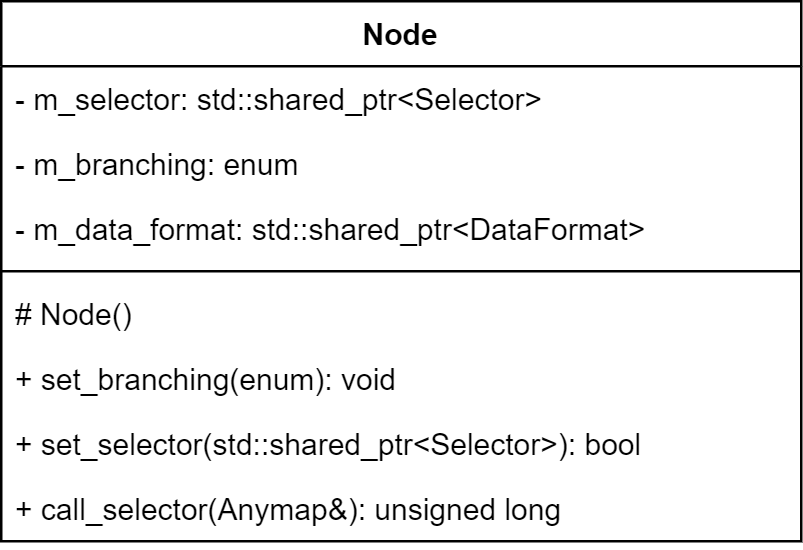
\includegraphics[width=\textwidth]{images/class.node.png}
			\caption{UML-диаграмма класса узла графа}
		\end{minipage}\hfill\begin{minipage}{0.49\textwidth}
			\begin{itemize}
				\item Использует умные указатели (\textsf{shared_ptr}) -- эффективное использование памяти.
				\item Защищённый конструктор -- объекты данного класса создаются только в пределах класса графовой модели.
				\item Интерфейс и информационные поля соответствуют требованиям.
			\end{itemize}
		\end{minipage}
	\end{figure}
\end{frame}
%%%%%%%%%%%%%%%%%%%%%%%%%%%%%%%%%%%%%%%%%%%%%%%%%%%%%%%%%%%%%%%%
\subsection{Предлагаемая структура данных ребра графовой модели}
%%%%%%%%%%%%%%%%%%%%%%%%%%%%%%%%%%%%%%%%%%%%%%%%%%%%%%%%%%%%%%%%
\begin{frame}%[allowframebreaks=0.9,t]
	\begin{figure}
		\begin{minipage}{0.49\textwidth}
			\begin{itemize}
				\item Использует умные указатели (\textsf{shared_ptr}) -- эффективное использование памяти.
				\item Защищённый конструктор -- объекты данного класса создаются только в пределах класса графовой модели.
				\item Интерфейс и информационные поля соответствуют требованиям.
				\item Для прохода по ребру необходимо назначить ему хотя бы одну пару предикат-обработчик (объединённых в структуру данных \textsf{Morphism}) с помощью метода set_function.
			\end{itemize}
		\end{minipage}\hfill\begin{minipage}{0.49\textwidth}
			\centering
			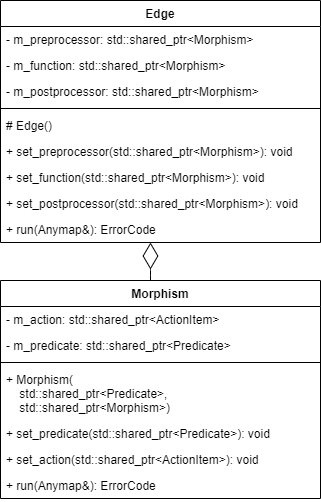
\includegraphics[height=0.75\textheight]{images/class.edge.png}
			\caption{UML-диаграмма класса ребра графа}
		\end{minipage}
	\end{figure}
\end{frame}

%%%%%%%%%%%%%%%%%%%%%%%%%%%%%%%%%%%%%%%%%%%%%%%%%%%%%%%%%%%%%%%%
\subsection{Предлагаемая структура данных графовой модели}
%%%%%%%%%%%%%%%%%%%%%%%%%%%%%%%%%%%%%%%%%%%%%%%%%%%%%%%%%%%%%%%%
\begin{frame}%[allowframebreaks=0.9,t]
	\begin{figure}
		\begin{minipage}{0.49\textwidth}
			\centering
			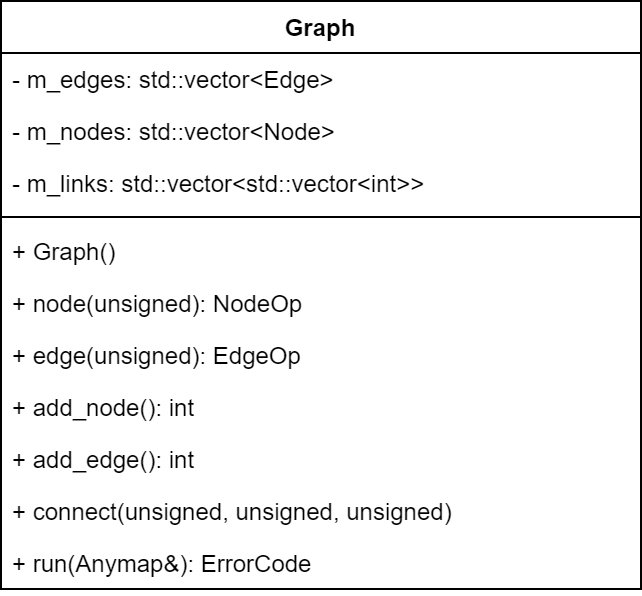
\includegraphics[width=0.8\textwidth]{images/class.graph.png}
			\caption{UML-диаграмма класса графа}
		\end{minipage}\hfill\begin{minipage}{0.49\textwidth}
			\begin{itemize}
				\item Хранит в себе узлы и рёбра графовой модели.
				\item Хранит в себе динамическую матрицу смежности.
				\item Позволяет добавлять узлы и рёбра и связывать их.
				\item Позволяет запустить обход графовой модели с заданным набором входных данных.
			\end{itemize}
		\end{minipage}
	\end{figure}
\end{frame}
%%%%%%%%%%%%%%%%%%%%%%%%%%%%%%%%%%%%%%%%%%%%%%%%%%%%%%%%%%%%%%%%
\subsection{Дополнительные структуры данных}
%%%%%%%%%%%%%%%%%%%%%%%%%%%%%%%%%%%%%%%%%%%%%%%%%%%%%%%%%%%%%%%%
\begin{frame}
	\begin{figure}
		\begin{minipage}{0.49\textwidth}
			\begin{itemize}
				\item NodeOp -- сокращение от ``Node Operation''.
				\item Дополнительная структура данных для операций с узлами.
				\item Хранит только индекс узла -- эффективное использование памяти.
				\item Позволяет получить соседние узлы для данного узла;
				\item Позволяет получить входящие и исходящие рёбра для данного узла;
				\item Позволяет при необходимости обратиться к интерфейсу самого узла.
			\end{itemize}
		\end{minipage}\hfill\begin{minipage}{0.49\textwidth}
			\centering
			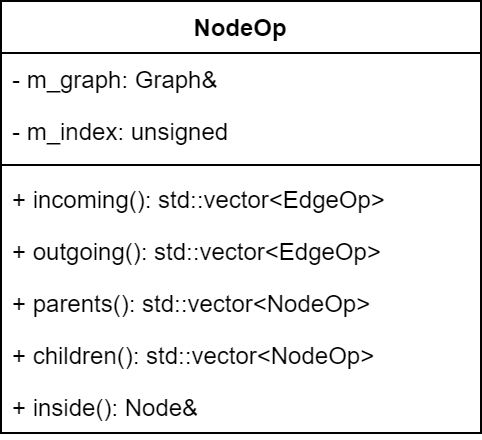
\includegraphics[width=0.75\textwidth]{images/class.nodeop.png}
			\caption{UML-диаграмма класса операции с узлом}
		\end{minipage}
	\end{figure}
\end{frame}

\begin{frame}
	\begin{figure}
		\begin{minipage}{0.49\textwidth}
			\begin{itemize}
				\item EdgeOp -- сокращение от ``Edge Operation''
				\item Дополнительная структура данных для операций с рёбрами.
				\item Хранит только индекс ребра -- эффективное использование памяти.
				\item Позволяет получить начальный и конечный узлы для данного ребра.
				\item Позволяет при необходимости обратиться к интерфейсу самого ребра.
			\end{itemize}
		\end{minipage}\hfill\begin{minipage}{0.49\textwidth}
			\centering
			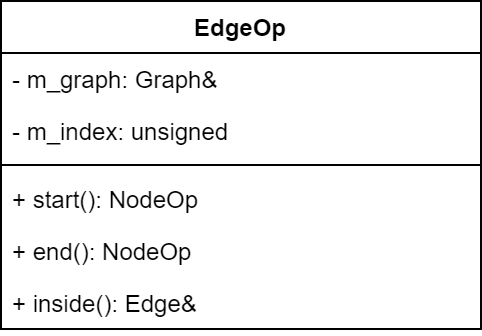
\includegraphics[width=0.75\textwidth]{images/class.edgeop.png}
			\caption{UML-диаграмма класса операции с ребром}
		\end{minipage}
	\end{figure}
\end{frame}
%%%%%%%%%%%%%%%%%%%%%%%%%%%%%%%%%%%%%%%%%%%%%%%%%%%%%%%%%%%%%%%%
